\begin{frame}
    \frametitle{Physics of what we calculate}

    \begin{columns}
        \column{0.4\textwidth}
            \begin{wideitemize}
                \item Content of my Practical Training (Fachpraktikum) \pause
                \item Hubbard Model Hamiltonian \pause
                \item System under influence of external electric field
            \end{wideitemize}

        \column{0.4\textwidth}
            \onslide
            \makebox[\textwidth][c]{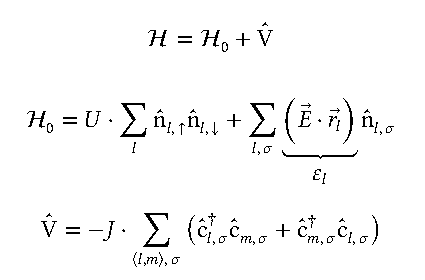
\includegraphics[width=\textwidth]{./main-content/physics/hamiltonian.pdf}}

    \end{columns}

    % notes 
    \onslide % on all slides of frame
    \note[item] {
        Hubbard-Model Hamiltonian with exterally applied electric field
    }
    \note[item] {
        Hard-Core Bosinic Operators (will be explained in later slide, do not need to elaborate on)
    }
    \note[item] {
        Spin-dependent lattice Model
    }
    \note[item] {
        External electric field acts symmetric on both spin directions 
        \begin{itemize}
            \item This will be important later, multiple times
            \item All terms always need to be symmetric in terms of spin up/down
        \end{itemize}
    }
\end{frame} 

\begin{frame}
    \frametitle{Physics of what we calculate}

    \begin{columns}
        \column{0.4\textwidth}
            \begin{wideitemize}
                \item 2-dimensional geometry
                \item Square lattice arrangement
                \item Computation for general size and field angle
            \end{wideitemize}
            
            \vspace{0.5cm}
            \pause
            \begin{itemize}
                \item[Goal:]
                Approximate evaluation of time-evolution using Monte-Carlo Sampling
            \end{itemize}

        \onslide
        \column{0.4\textwidth}
            \makebox[\textwidth][c]{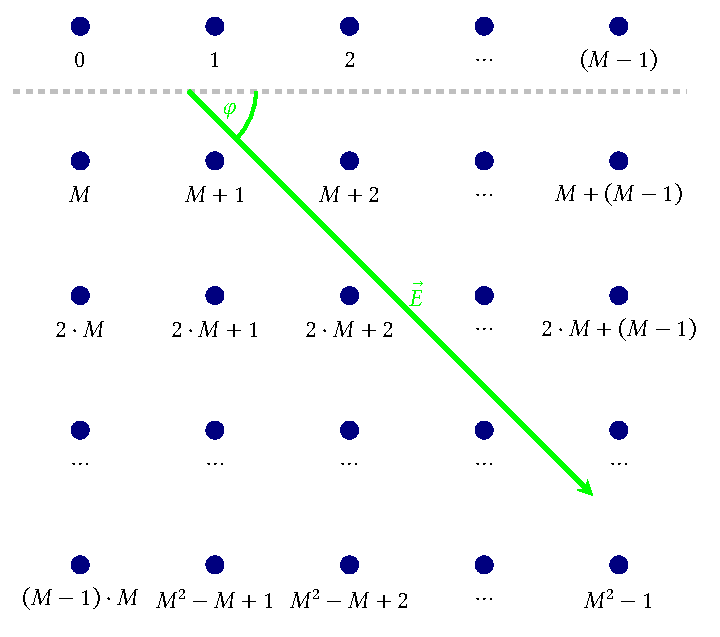
\includegraphics[width=.9\textwidth]{./main-content/physics/geometry.pdf}}
            
    \end{columns}

    % notes 
    \onslide % on all slides of frame
    \note[item] {
        2-dimensional square geometry
    }
    \note[item] {
        Program supports already for general size inputs
    }
    \note[item] {
        Thanks to the Monte-Carlo Sampling we can even efficiently evaluate larger systems already
    }
\end{frame}

\begin{frame}
    \frametitle{Physics of what we calculate}

    \begin{columns}
        \column{0.4\textwidth}
            \begin{wideitemize}
                \item Hard-Core Bosonic operators
                \onslide<2->
                \begin{itemize}
                    \item (Would work analogously with Fermionic operators)
                \end{itemize}
                \onslide<3->
                \item Two spin-degrees of freedom rewritten in alternate notation
            \end{wideitemize}

        \column{0.4\textwidth}
            \onslide
            \makebox[\textwidth][c]{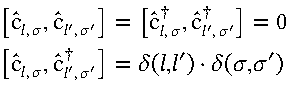
\includegraphics[page=1,width=.75\textwidth]{./main-content/physics/rewrite.pdf}}
            \onslide<3->
            \makebox[\textwidth][c]{\includegraphics[page=2,width=.75\textwidth]{./main-content/physics/rewrite.pdf}}
            \makebox[\textwidth][c]{\includegraphics[page=3,width=.75\textwidth]{./main-content/physics/rewrite.pdf}}
            
    \end{columns}
    
    % notes 
    \onslide % on all slides of frame
    \note[item] {
        Operators are hard-core bosonic
        \begin{itemize}
            \item standard commutation relations
            \item occupations are only either zero ore one
        \end{itemize}
    }
    \note[item] {
        fermionic operators (anti-commutation) would work equivalent
    }
    \note[item] {
        other notation to rewrite the two spin degrees of freedom into two operators of different dof makes it more readable and comfortable to apply computationally in some cases
    }
\end{frame}

